\documentclass[a4paper]{article}
\input{~/preamble.tex}

\title{Συστήματα Αναμονής \\ 4η εργαστηριακή άσκηση}
\author{Νικόλαος Παγώνας, el18175}
\date{}

\begin{document}

\maketitle

\subsection*{Ανάλυση και Σχεδιασμός τηλεφωνικού κέντρου}

\subsubsection*{(1)}

Σχεδιάζουμε το διάγραμμα ρυθμού μεταβάσεων για το σύστημα M/M/c/c:

\begin{figure}[H]
	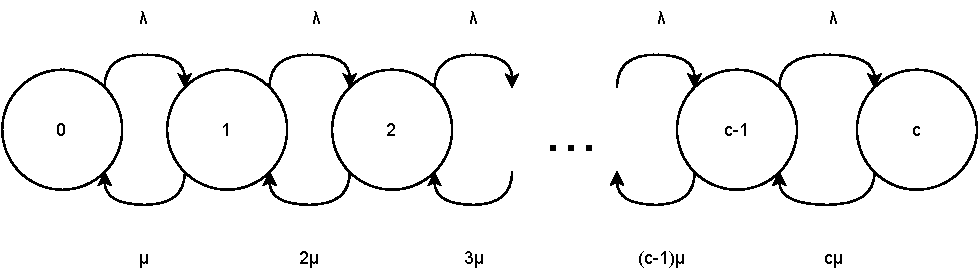
\includegraphics[width=\textwidth]{transition_diagram_1.pdf}
\end{figure}

Με βάση το παραπάνω διάγραμμα, διατυπώνουμε τις τοπικές εξισώσεις ισορροπίας:

\begin{align*}
	P_k &= \frac{\lambda}{k \mu} P_{k-1} \\
	    &= \frac{\lambda}{k \mu} \cdot \frac{\lambda}{(k-1) \mu} \cdot \frac{\lambda}{(k-2) \mu} \cdots \frac{\lambda}{2 \mu} \cdot \frac{\lambda}{\mu} \cdot P_0 \\
	    &= \frac{1}{k!}\left(\frac{\lambda}{\mu}\right)^k P_0 \\
	    &= \frac{\rho^k}{k!} P_0
\end{align*}

Και λόγω της ιδιότητας της κανονικοποίησης:


\[
	\scalebox{1.5}{$\sum\limits_{k=0}^c$} P_k = 1 \implies \\
	\scalebox{1.5}{$\sum\limits_{k=0}^c$} \frac{\rho^k}{k!}P_0 = 1 \implies \\
	P_0 = \frac{1}{\scalebox{1.5}{$\sum\limits_{k=0}^c$} \dfrac{\rho^k}{k!}} \implies\\
	\boxed{P_c = P_{blocking} = \frac{\rho^c/c!}{\scalebox{1.5}{$\sum\limits_{k=0}^c$} \dfrac{\rho^k}{k!}}}
\]


Επομένως:
\begin{align*}
	\text{Μέσος ρυθμός απωλειών } &= \lambda - \text{\gamma}\\ 
	&=\lambda \cdot P_{\text{blocking}} \\ 
	&= \lambda \cdot \frac{\rho^c/c!}{\scalebox{1.5}{$\sum\limits_{k=0}^c$} \dfrac{\rho^k}{k!}}
\end{align*}

Τέλος, υλοποιούμε την συνάρτηση \texttt{erlangb\_factorial}, η οποία υπολογίζει το 
\[
	B(ρ,c) = \frac{ρ^c/c!}{\scalebox{1.5}{ $ \sum_{k=0}^c \frac{ρ^k}{k!} $ }} \text{, ως εξής:}
\]

\lstinputlisting[language=Octave]{erlangb_factorial.m}

Η ορθή λειτουργία επαληθεύτηκε με χρήση της συνάρτησης \texttt{erlang} του πακέτου \texttt{queueing}.

\subsubsection*{(2)}

Τώρα θα υλοποιήσουμε ξανά την παραπάνω συνάρτηση, αυτή τη φορά με επαναληπτικό τρόπο. Ονομάζουμε την νέα υλοποίηση \texttt{erlangb\_iterative}:

\lstinputlisting[language=Octave]{erlangb_iterative.m}

Και πάλι ελέγχουμε την ορθότητα μέσω της συνάρτησης \texttt{queueing/erlang}.

\subsubsection*{(3)}

Αν τρέξουμε τις συναρτήσεις \texttt{erlangb\_factorial} και \texttt{erlangb\_iterative} με παραμέτρους ρ=c=1024, παρατηρούμε ότι η πρώτη επιστρέφει \texttt{NaN} (Not a Number). Αυτό συμβαίνει διότι για το Octave, $ 1024^{1024} $ = Inf και 1024! = Inf, οπότε έχουμε διαίρεση Inf/Inf η οποία επιστρέφει NaN. Αντίθετα, η δεύτερη επιστρέφει το σωστό αποτέλεσμα (0.024524), γιατί ο αλγόριθμος είναι επαναληπτικός και διατηρεί τις τιμές του σε λογικά όρια, από μετάβαση σε μετάβαση.

\subsubsection*{(4)}

\subsubsection*{(a)}

Μία μοντελοποίηση για έναν πελάτη (όχι η μοναδική) είναι να θεωρήσουμε: 
\[
	λ = 1 \ \frac{\text{κλήση}}{\text{ώρα}} \text{ και } \frac{1}{μ} = 23 \frac{\text{λεπτά}}{\text{κλήση}}
\]

Έτσι, 
\[
	ρ_1 = \frac{λ}{μ} = 1 \ \frac{\text{κλήση}}{\text{ώρα}} \cdot 23 \ \frac{\text{λεπτά}}{\text{κλήση}} = \frac{\text{1 κλήση}}{\text{60 λεπτά}} \cdot \frac{\text{23 λεπτά}}{\text{1 κλήση}} = \frac{23}{60} \ Erlangs.
\]
 
Για 200 πελάτες έχουμε:

\[
	 ρ_{200} = 200 \cdot ρ_1 = 76.67 \ Erlangs.
\]

\subsubsection*{(b)}

Απεικονίζουμε την πιθανότητα απόρριψης πελάτη συναρτήσει του αριθμού των τηλεφωνικών γραμμών (1...200):

\begin{figure}[H]
	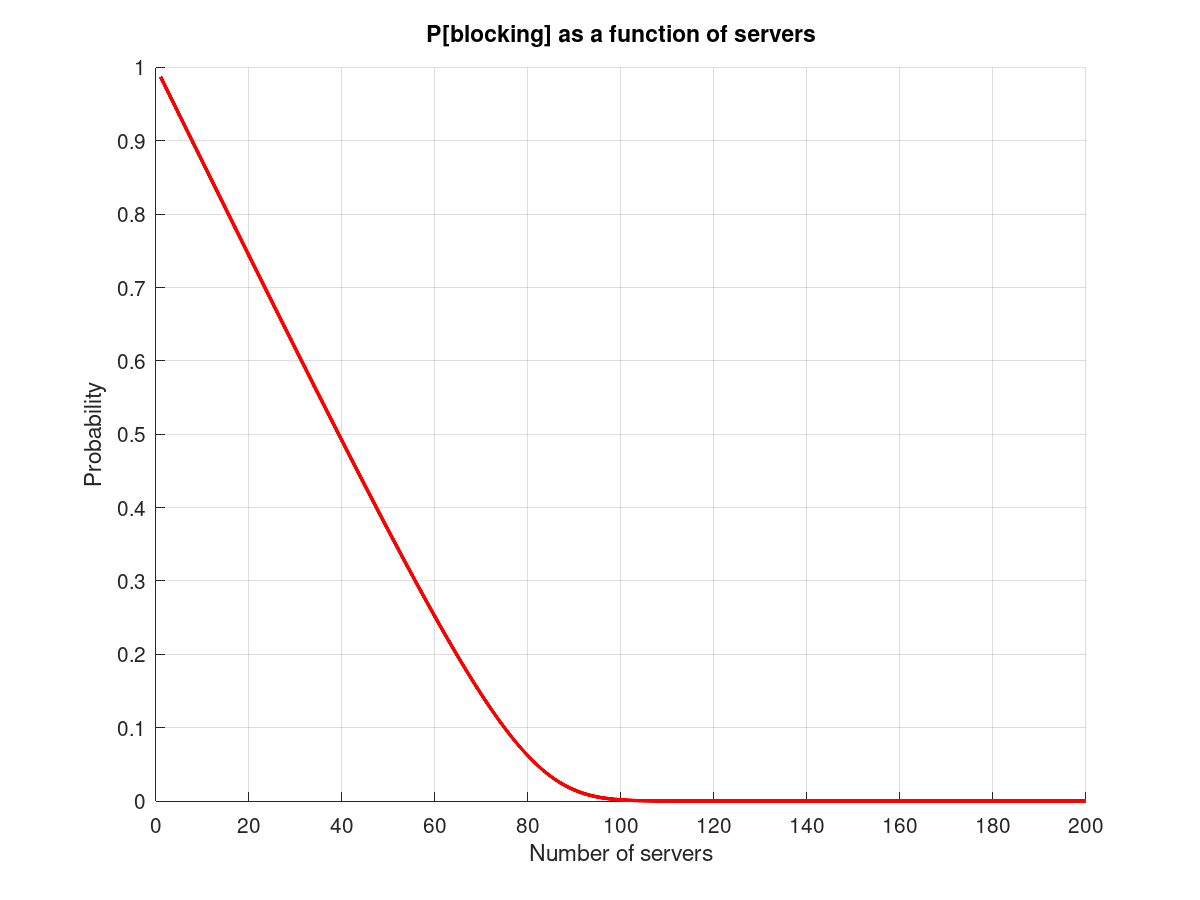
\includegraphics[width=\textwidth]{call_center.png}
\end{figure}

\subsubsection*{(c)}

Ο ελάχιστος αριθμός τηλεφωνικών γραμμών που χρειαζόμαστε προκειμένου να έχουμε πιθανότητα απόρριψης μικρότερη του 1\% είναι 93 εξυπηρετητές, οι οποίοι δίνουν P[blocking] = 0.00836795 (0.83\%).

\subsection*{Κώδικας που χρησιμοποιήθηκε για το ερώτημα 4}

\lstinputlisting[language=Octave]{call_center.m}

\subsection*{Σύστημα εξυπηρέτησης με δύο ανόμοιους εξυπηρετητές}

\subsubsection*{(1)}

Σχεδιάζουμε το διάγραμμα ρυθμών μεταβάσεων του συστήματος στην κατάσταση ισορροπίας:

\begin{figure}[H]
	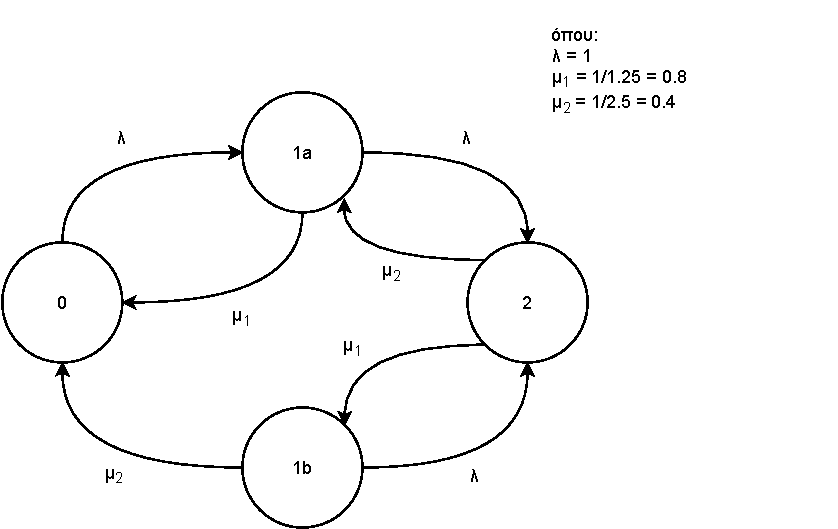
\includegraphics[width=\textwidth]{transition_diagram_2.pdf}
\end{figure}

Για τις εξισώσεις ισορροπίας παίρνουμε την τομή που περικλείει μόνο τον κόμβο 0, την τομή που περικλείει μόνο τον κόμβο 1a και την τομή που περικλείει μόνο τον κόμβο 1b, καθώς και την ιδιότητα της κανονικοποίησης, οπότε έχουμε: 

\begin{align}
	1 \cdot P_0 &= 0.8 \cdot P_{1a} + 0.4 \cdot P_{1b}	\\
	0.8 \cdot P_{1a} + 1 \cdot P_{1a} &= 1 \cdot P_0 + 0.4 \cdot P_2 \\
	1 \cdot P_{1b} + 0.4 \cdot P_{1b} &= 0.8 \cdot P_2	\\
	P_0 + P_{1a} + P_{1b} + P_{2} &= 1	 
\end{align}

Λύνοντας το παραπάνω 4x4 σύστημα προκύπτουν: 
\[
	P_0 = 0.24951, P_{1a} = 0.21442, P_{1b} = 0.19493, P_2 = 0.34113
\]

Επομένως, 
\[
	P[\text{blocking}] = P_2 = 0.34113 = 34.1 \%
\]

Για τον μέσο αριθμό πελατών στο σύστημα ισχύει: 

\[
	E[n] = 0 \cdot P_0 + 1 \cdot (P_{1a} + P_{1b}) + 2 \cdot P_2 = 1.09161 \text{ πελάτες}
\]

\subsubsection*{(2)}

Για τα κατώφλια έχουμε: 

\begin{align*}
	\text{threshold\_1a} &= \frac{λ}{λ + μ_1} \\ 
	\text{threshold\_1b} &= \frac{λ}{λ + μ_2} \\
	\text{threshold\_2\_first} &= \frac{λ}{λ + μ_1 + μ_2} \\ 
	\text{threshold\_2\_second} &= \frac{λ+μ_1}{λ + μ_1 + μ_2} \\ 
\end{align*}

Η λογική είναι ότι στα threshold 1a,1b και 2\_first, όσο μεγαλύτερο είναι το λ, τόσο μεγαλύτερη και η πιθανότητα ο τυχαίος αριθμός να πέσει μέσα στο διάστημα [0,threshold]. Το threshold\_2\_second έχει φτιαχτεί έτσι ώστε να χωρίσουμε το διάστημα [0,1] σε τρία κομμάτια: 

\begin{itemize}
	\item $ \left[0\ \ ,\ \ \dfrac{λ}{λ+μ_1+μ_2}\right] $
	\item $ \left[\dfrac{λ}{λ+μ_1+μ_2}\ \ ,\ \ \dfrac{λ+μ_1}{λ+μ_1+μ_2}\right] $
	\item $ \left[\dfrac{λ+μ_1}{λ+μ_1+μ_2}\ \ ,\ \  1\right] $,
\end{itemize}  

Τα οποία έχουν μήκος $ \dfrac{λ}{λ+μ_1+μ_2} ,\ \dfrac{μ_1}{λ+μ_1+μ_2} \ \text{ και }\ \dfrac{μ_2}{λ+μ_1+μ_2}$ αντίστοιχα.

Γενικά για κάθε κατάσταση, χωρίζουμε το διάστημα [0,1] σε τόσα υποδιαστήματα, όσες και οι διαφορετικές καταστάσεις στις οποίες μπορούμε να πάμε από την κατάσταση αυτή.

Το κριτήριο σύγκλισης είναι:

\begin{verbatim} 
if abs(mean_clients - previous_mean_clients) < 0.00001
    break;
endif
\end{verbatim}

Στην ουσία ελέγχουμε ανά 1000 μεταβάσεις (\texttt{if mod(time, 1000) == 0}) αν ο μέσος αριθμός πελατών αλλάζει πολύ λίγο (κατά 0.00001), δηλαδή αν έχουμε σύγκλιση.  

Οι πιθανότητες που προκύπτουν από το πρόγραμμα είναι:

\verbatiminput{simulation_results.txt}

oι οποίες συμφωνούν κατά πολύ μεγάλο βαθμό με τις θεωρητικές πιθανότητες που υπολογίστηκαν στο προηγούμενο ερώτημα.

\subsection*{Κώδικας που χρησιμοποιήθηκε για την προσομοίωση, με συμπληρωμένα τα κενά}

\lstinputlisting[language=Octave]{two_servers.m}

\end{document}
